\documentclass[tikz, border=5pt]{standalone}

\begin{document}

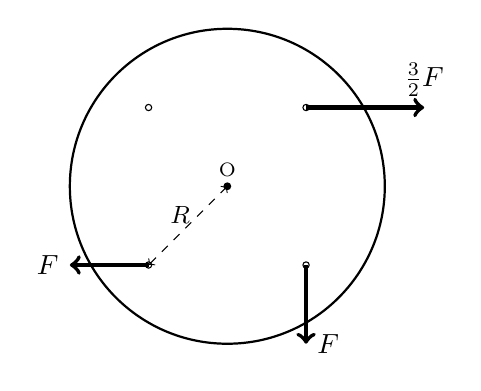
\begin{tikzpicture}

    %% Original

    % Plate
    \draw[thick] (0,0) circle (2);
    \draw[<->, dashed] (0,0) -- (-1,-1) node[pos=0.6, above] {\small \(R\)};
    \fill[black] (0,0) circle (0.05);
    \node[above] at (0,0) {\scriptsize O};

    % Square points
    \draw (1,1) circle (0.04);
    \draw (1,-1) circle (0.04);
    \draw (-1,1) circle (0.04);
    \draw (-1,-1) circle (0.04);

    % Forces
    \draw[->, line width=1.5pt] (1,1) -- ++(1.5,0) node[above] {\(\frac{3}{2} F\)};
    \draw[->, line width=1.5pt] (1,-1) -- ++(0,-1) node[right] {\(F\)};
    \draw[->, line width=1.5pt] (-1,-1) -- ++(-1,0) node[left] {\(F\)};

\end{tikzpicture}

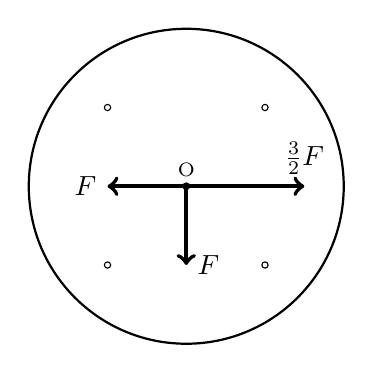
\begin{tikzpicture}

    %% Net force

    % Plate
    \draw[thick] (0,0) circle (2);
    \fill[black] (0,0) circle (0.05);
    \node[above] at (0,0) {\scriptsize O};

    % Square points
    \draw (1,1) circle (0.04);
    \draw (1,-1) circle (0.04);
    \draw (-1,1) circle (0.04);
    \draw (-1,-1) circle (0.04);

    % Forces
    \draw[->, line width=1.5pt] (0,0) -- ++(1.5,0) node[above] {\(\frac{3}{2} F\)};
    \draw[->, line width=1.5pt] (0,0) -- ++(0,-1) node[right] {\(F\)};
    \draw[->, line width=1.5pt] (0,0) -- ++(-1,0) node[left] {\(F\)};

\end{tikzpicture}

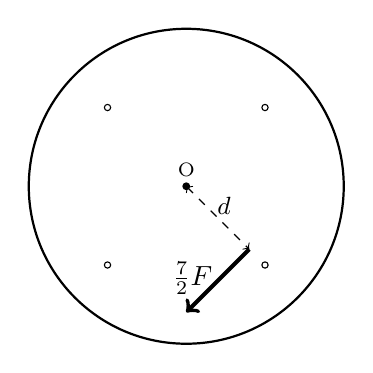
\begin{tikzpicture}

    %% Net torque

    % Plate
    \draw[thick] (0,0) circle (2);
    \draw[<->, dashed] (0,0) -- (0.8,-0.8) node[pos=0.6, above] {\small \(d\)};
    \fill[black] (0,0) circle (0.05);
    \node[above] at (0,0) {\scriptsize O};

    % Square points
    \draw (1,1) circle (0.04);
    \draw (1,-1) circle (0.04);
    \draw (-1,1) circle (0.04);
    \draw (-1,-1) circle (0.04);

    % Forces
    \draw[->, line width=1.5pt] (0.8,-0.8) -- ++(-0.8,-0.8) node[pos=0.9, above] {\(\frac{7}{2}F\)};

\end{tikzpicture}

\end{document}
